\documentclass[handout]{beamer}
\usepackage{textpos}
\usepackage{listings}
\usepackage{hyperref}

\usepackage{caption}
\captionsetup[table]{labelformat=empty}

\usepackage{xcolor}
\definecolor{mygreen}{rgb}{0,0.6,0}
\definecolor{mygray}{rgb}{0.5,0.5,0.5}

\usepackage{graphicx}% http://ctan.org/pkg/graphicx
\usepackage{booktabs}

\lstset{language=C++,
           basicstyle=\ttfamily\scriptsize,
           keywordstyle=\color{blue}\ttfamily,
           stringstyle=\color{red}\ttfamily,
           commentstyle=\color{mygreen}\ttfamily,
          breaklines=true,
          captionpos=b,
          numbers=left,
          numbersep=5pt,
          numberstyle=\tiny\color{mygray},
          rulecolor=\color{black},
          xleftmargin=\parindent,
          frame=single,
          backgroundcolor=\color{white}
}

\setbeamercolor{normal text}{fg=black,bg=white}
\definecolor{beamer@blendedblue}{rgb}{0,0,0}
\setbeamercolor{structure}{fg=beamer@blendedblue}

\title{Working with Device Memory}
\author{
    \includegraphics[width=3cm]{../media/logo/NVLogo_2D.eps}
    \vspace{0.75cm}
    \\}
\date{\today}

\begin{document}

\frame{\titlepage}

%\section[Outline]{}
\begin{frame}{Outline}
\tableofcontents
\end{frame}

\addtobeamertemplate{frametitle}{}{%
\begin{textblock*}{200mm}(.75\textwidth,-0.35cm)
\includegraphics[width=3cm]{../media/logo/NVLogo_2D_H.eps}
\end{textblock*}}

\addtobeamertemplate{navigation symbols}{}{%
    \usebeamerfont{footline}%
    \usebeamercolor[fg]{footline}%
    \hspace{1em}%
    \insertframenumber/\inserttotalframenumber
}

\section{Introduction}
\begin{frame}{Memory Considerations}
There are two primary aspects of memory management when working with accelerators:
\hfill\break
\begin{itemize}
\itemsep1em
    \item<1->Since the GPU is a physically separate device connected to the host via PCI-e bus, the host and device memories have separate address spaces.
    \item<1->As a throughput oriented compute architecture, the GPU device itself provides five distinctly different memory types for use in kernel development and execution.
\end{itemize}
\hfill\break
Many features in each CUDA release are centralized around robustification of the host/device memory interaction while mastery of the various device memory types is both an art and a science essential to every GPU accelerated application.
\end{frame}

\begin{frame}{Programable Memory Hierarchy}
\begin{itemize}
	\item<1->Both the CPUs and GPU compute devices use similar principles and models in memory hierarchy design (i.e. progressively lower-latency but lower capacity memories to optimize performance).
	\item<1->The key difference in the GPU memory model is that CUDA programing exposes more of the device memory hierarchy and provides explicit programable control. 
\end{itemize}
\end{frame}

\begin{frame}{Device Memory Layout}
\begin{figure}
\begin{center}
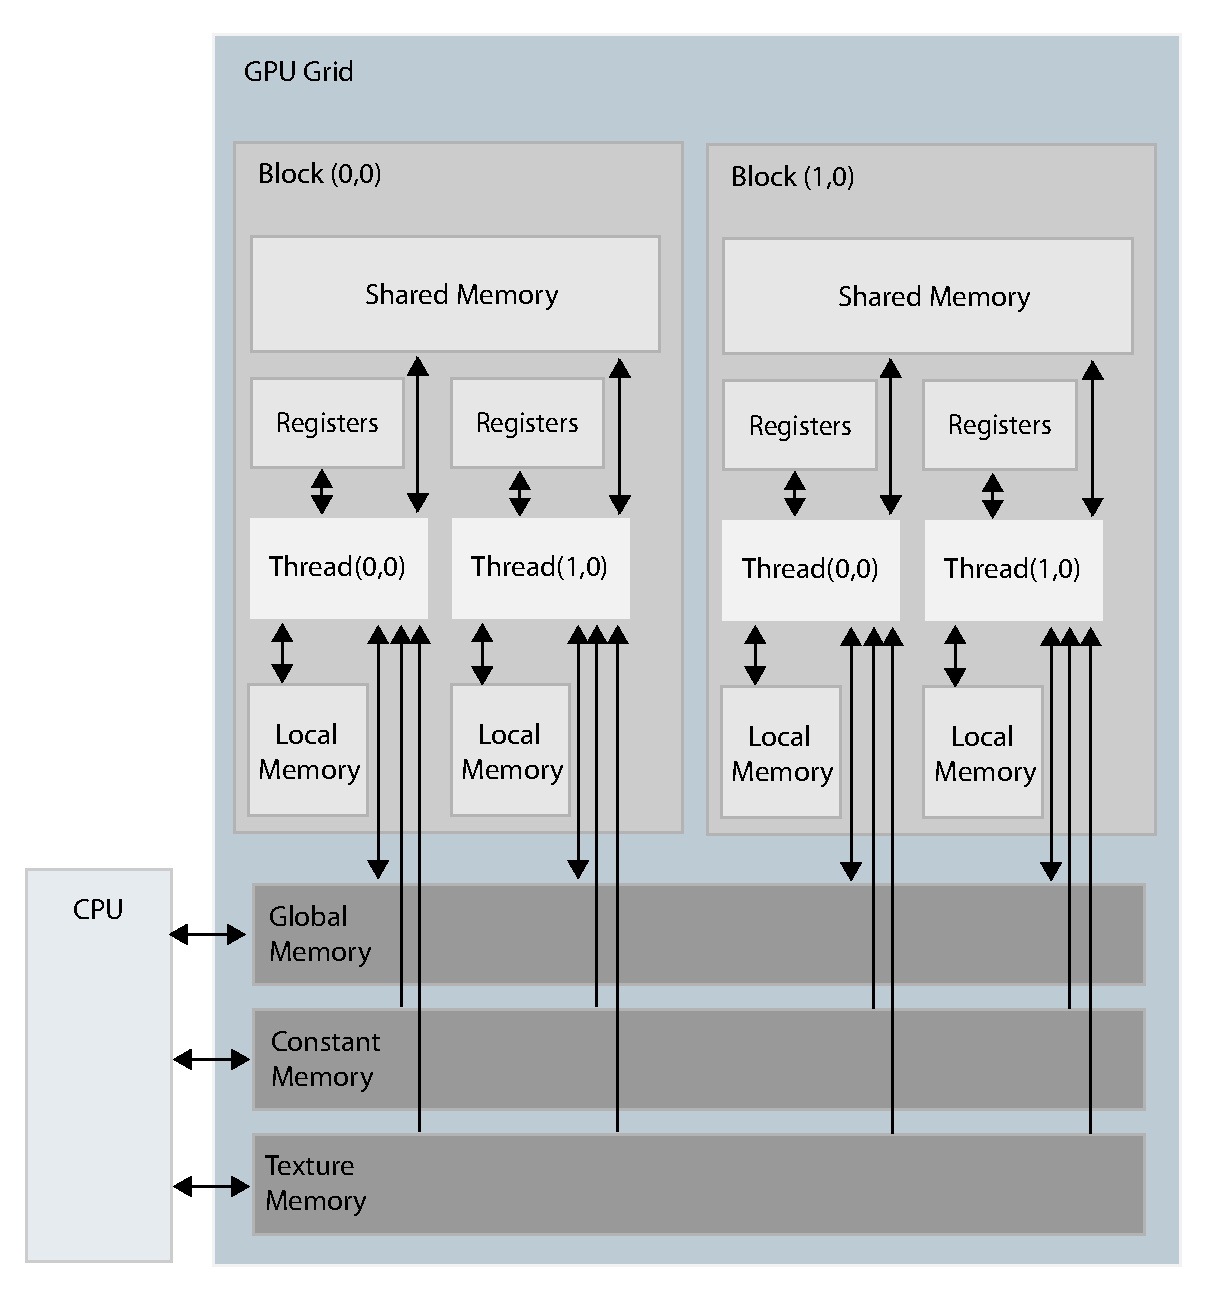
\includegraphics[width=6cm]{../media/cuda_mem.pdf}
\caption{Various programable device memories.  The host can only access global, constant, and texture memories.  Each SM has a limited amount of shared memory which is partitioned among resident thread-blocks while registers are thread exclusive.}
\end{center}
\end{figure}
\end{frame}

\begin{frame}{Device Global Memory}
\begin{itemize}
	\item<1->Global memory is the largest host accessible memory available on the device which is accessible to all threads in any block.  
	\item<1->Global memory is off the processor chip (implies long access latencies) and is implemented using dynamic random access memory (DRAM) technologies such as double data rate type five synchronous graphics memory (GDDR5).
	\item<1->Global memory is generally referred to as just \emph{device memory} and is usually on the order of 6 to 12 GB in size.
	\item<1->Since device memory is directly attached and accessed using a dedicated memory controller integrated into the GPU, the peak bandwidth is extremely high (typically 100 to 300 GB/s). 
	\item<1->The next generation Pascal P100 accelerator leverages a manufacturing technique called Chip-on-Wafer-on-Substrate (CoWoS) with second generation high bandwidth memory (HBM2) technology (i.e. stacked DRAM) achieving over 700 GB/s memory bandwidth.
\end{itemize}
\end{frame}

\begin{frame}{Device Global Memory}
\begin{itemize}
	\item<1->Whenever runtime API calls such as {\fontfamily{qcr}\selectfont cudaMalloc}, {\fontfamily{qcr}\selectfont cudaFree} and {\fontfamily{qcr}\selectfont cudaMemcpy} are invoked, global memory is being referenced.
	\item<1->Device global memory is accessed in CUDA kernels using \emph{device pointers} which reside in the \emph{device address space}.  
	\item<1->Host code can perform pointer arithmetic on device pointers but can not generally dereference them.  
	\item<1->Keep in mind that mapped pinned pointers are located in host memory but can be accessed by the GPU (i.e. zero-copy).  Although, on non-UVA systems, the host and device pointers to this memory are different and {\fontfamily{qcr}\selectfont cudaGetDevicePointer()} must be used to map host pointers to corresponding device pointers.  But when UVA is in effect, the pointers are the same.
\end{itemize}
\end{frame}


\begin{frame}[fragile]{Device Global Memory}
\begin{lstlisting}[caption={Device global memory accessed by CUDA kernel using device pointer.  This kernel writes the integer {\fontfamily{qcr}\selectfont value} into the address range given by {\fontfamily{qcr}\selectfont array} and {\fontfamily{qcr}\selectfont N}.  The references to {\fontfamily{qcr}\selectfont blockIdx}, {\fontfamily{qcr}\selectfont blockDim} and {\fontfamily{qcr}\selectfont gridDim} enable the kernel to operate correctly for each individual thread with whatever block and grid parameters were used in the kernel launch.}] 
__global__ void GPUmemset(int *array, int value, size_t N)
{
    for (int i = blockIdx.x*blockDim.x + threadIdx.x;
          i < N;
          i += gridDim.x*blockDim.x)
    {
          array[i] = value;
    }
}
\end{lstlisting}
\end{frame}

\begin{frame}{Error Correcting Codes (ECC)}
\begin{itemize}
	\item<1->Tesla GPUs (SM 2.x and later) have the ability to run with error correction.  Devices with ECC enabled can silently correct single-bit errors and report double-bit errors.
	\item<1->ECC can be queried, enabled, and disabled using the {\fontfamily{qcr}\selectfont nvidia-smi} command-line tool or the NVIDIA Management Library (\href{https://developer.nvidia.com/nvidia-management-library-nvml}{\color{blue}NVML}) C-based API directly.
	\item<1->ECC consumes a portion of global memory ($\approx$ 12\%), used to store redundancy, and reduces the overall memory bandwidth ($\approx$ 20\%) due to the additional traffic for memory checksums.  The exact impact of ECC on bandwidth depends on the memory access pattern.
	\item<1->Note that ECC coverage extends to other memories on the device such as L2/L1 cache and register file space.  However, facilities such as hardware queues, thread block scheduler, warp scheduler, instruction dispatch unit, etc are not covered by ECC.
\end{itemize}
\end{frame}

\begin{frame}{Error Correcting Codes (ECC)}
\begin{itemize}
	\item<1->ECC status can be queried via the runtime API via device property {\fontfamily{qcr}\selectfont ECCEnabled} and/or driver API device attribute {\fontfamily{qcr}\selectfont CU\_DEVICE\_ATTRIBUTE\_ECC\_ENABLED} which are 1 if the device has ECC support turned on, or 0 otherwise.
	\item<1->When an uncorrectable ECC error is detected, CUDA runtime calls will return {\fontfamily{qcr}\selectfont cudaErrorECCUncorrectable} while the driver API returns {\fontfamily{qcr}\selectfont CUDA\_ERROR\_ECC\_UNCORRECTABLE}.  
	\item<1->No notification of ECC errors is available within a CUDA kernel. ECC errors are reported, by the driver to the host, once the launch has completed. Any ECC errors which arise during execution of a nested program (i.e. kernel launch within a kernel) will either generate an exception or continue execution (depending upon error and configuration).
	\item<1->With ECC enabled, the memory error events will be recorded in the InfoROM for retrieval (typically using {\fontfamily{qcr}\selectfont nvidia-smi}).
\end{itemize}
\end{frame}

\begin{frame}{Error Correcting Codes (ECC)}
\begin{itemize}
	\item<1->It is very important to note that typically a single instance of a single-bit-error (SBE) will be silently corrected on-the-fly by the device and thus requiring no user intervention.
	\item<1->However, once a double-bit-error (DBE) has been detected and flagged a {\fontfamily{qcr}\selectfont cudaErrorECCUncorrectable} will be triggered and all further execution on the device will be halted. 
	\item<1->An uncorrectable ECC error will cause the device context to become unusable and, in fact, the device becomes unusable until a reset is performed, or the driver is unloaded/reloaded (which effectively resets the GPU).  Therefore all subsequent kernel launch attempts will fail until a reset occurs.
	\item<1-> If ECC is not enabled, then execution will always continue, even in the presence of memory errors.
	\item<1->The ECC mechanism is not guaranteed to flag or detect errors more complex than a double-bit-error.
\end{itemize}
\end{frame}

\begin{frame}{Error Correcting Codes (ECC)}
\begin{itemize}
	\item<1->Depending on the memory access pattern, a single flipped bit may cause the error counters to increment more than once.
	\item<1->It is possible that multiple single-bit-errors could trigger {\fontfamily{qcr}\selectfont cudaErrorECCUncorrectable}
	\item<1->There is currently no way to artificially induce {\fontfamily{qcr}\selectfont cudaErrorECCUncorrectable} for testing purposes.
	%\item<1->Unfortunately, there is currently no way recover from a {\fontfamily{qcr}\selectfont cudaErrorECCUncorrectable} from within the CUDA runtime API -- the program must terminate. 
	\item<1->Note that double-bit ECC errors are additionally reported as \href{http://docs.nvidia.com/deploy/xid-errors/index.html}{\color{blue}XID errors} by the driver to the operating system kernel/event log (i.e. {\fontfamily{qcr}\selectfont /var/log/messages}).
	\item<1->The NVIDIA Validation Suite (\href{http://docs.nvidia.com/deploy/nvvs-user-guide/index.html}{\color{blue}NVVS}) is a health check and stress test tool provided as part of the \href{https://developer.nvidia.com/gpu-deployment-kit}{\color{blue}GPU Deployment Kit}. The NVVS tool facilitates checks for basic GPU health, including the presence of ECC errors, PCIe problems, bandwidth issues, and other general problems. 
\end{itemize}
\end{frame}

\begin{frame}{ECC Error Rates at Oak Ridge}
\begin{itemize}
%\itemsep1em
	\item<1->The Oak Ridge TITAN Supercomputer was the first GPU based supercomputer to perform over 10 petaFLOPS.
	\item<1->TITAN includes 18,688 Tesla GPUs and was ranked number 1 on the TOP500 when it became operational on Oct 29, 2012. 
	\item<1->Total combined GPU memory capacity is roughly 112TB.
	\item<1->TITAN sees on average one double-bit GPU memory error per week over all devices.
	\item<1->See \href{http://on-demand.gputechconf.com/gtc/2015/presentation/S5566-James-Rogers.pdf}{\color{blue}full report} by NCCS director Jim Rogers: \emph{GPU Errors on HPC Systems: Characterization, Quantification, and Implications for Architects and Operations}. 
	\item<1->See also \href{http://www4.ncsu.edu/~dtiwari2/Papers/2015_HPCA_Tiwari_GPU_Reliability.pdf}{\color{blue}Tiwari et al}, \emph{Understanding GPU Errors on Large-scale HPC Systems and the Implications for System Design and Operation}.
\end{itemize}
\end{frame}

\begin{frame}{Dynamic Page Retirement}
\begin{itemize}
	\item<1->The NVIDIA driver supports ``retiring'' of bad framebuffer memory cells from device global memory.  Read the \href{http://docs.nvidia.com/deploy/dynamic-page-retirement/index.html}{\color{blue}docs}.
	\item<1->The act of marking a memory cell for exclusion is called ``retiring'', while the act of actually excluding the associated page from memory allocations is called ``blacklisting''.
	\item<1->The device driver will retire a cell after a single instance of a double-bit ECC error or two instances of a single-bit ECC error. The addresses of memory pages with retired cells are stored in the device InfoROM.
	\item<1->When each device is initialized, the driver will retrieve retired page addresses from the InfoROM.  These retired addresses are then provided to the framebuffer manager for blacklisting such that they cannot be used by the driver.
	
\end{itemize}
\end{frame}

\begin{frame}[fragile]{Dynamic Page Retirement}
\begin{itemize}
\itemsep1em
	\item<1->This dynamic memory cell retirement strategy can improve the longevity of an otherwise good board and is thus an important resiliency feature on supported products.
	\item<1->Dynamic page retirement is available on all driver-supported Linux and Windows TCC platforms provided:
	\begin{itemize}
		\item<1->Driver version R319 and newer
		\item<1->K20 and newer Tesla enterprise products
	\end{itemize}
	\item<1->Dynamic page retirement is not supported on any NVIDIA Quadro, GRID or Geforce products.
	\item<1->Both XID errors in system logs and {\fontfamily{qcr}\selectfont nvidia-smi} provide visibility into page retirement.  For example
\end{itemize}
\begin{lstlisting}
    nvidia-smi -i <target gpu> -q -d  PAGE_RETIREMENT
\end{lstlisting}
\end{frame}

\begin{frame}{Dynamic Page Retirement}
\begin{itemize}
	\item<1->Marking cells for retirement will only occur when ECC is enabled. However, once a cell has been retired the associated page will \emph{always} be blacklisted by the driver, even if ECC is later disabled.
	\item<1->However, page retirement itself can \emph{never} be disabled. All previously retired pages will continue to be excluded in every future allocation. 
	\item<1->The SBE recurrence threshold for cell retirement is not configurable (i.e. always 2).   
	\item<1->The size of each blacklisted page is 4 KB and does reduce total available memory. 
	\item<1->A maximum of 192 retired cell addresses can be stored in the InfoROM but limited to 60 blacklisted pages at any one time. 
	\item<1->The maximum total size of blacklisted memory is $\approx$ 256 KB. 
\end{itemize}
\end{frame}

\begin{frame}{Global Memory: Coalescence}
\begin{itemize}
	\item<1->For best performance when reading and writing global memory, CUDA kernels must perform coalesced\footnote{Definition: co$\cdot$a$\cdot$lesce: come together and form one mass or whole.\hfill\break} memory transactions.
	\item<1->Recall that instructions are dispatched on a per-warp basis.  Therefore, when a warp performs a load/store, the number of memory transactions needed to satisfy the instruction depends on two factors:
	\begin{itemize}
		\item<1->Distribution of memory addresses across the 32 threads/warp.
		\item<1->Alignment of memory addresses per transaction.
	\end{itemize} 
	\item<1->In general, fewer memory transactions needed to fulfill a load/store instruction across a warp means better kernel perf. 
	\item<1->For SM 2.x and later, achieving load/store memory throughput efficiency is more relaxed because memory transactions are cached in L1/L2. 
\end{itemize}
\end{frame}

\begin{frame}{Global Memory: Coalescence}
\begin{itemize}
\itemsep1em
	\item<1->Memory transactions are coalesced on a per-warp basis.
	\item<1->There is a (simplified) set of criteria for reads and writes performed by a warp to be coalesced:
	\hfill\break
	\begin{enumerate}
	\itemsep1em
		\item<1->The words must be at least 32 bits in size.  Reading or writing 8-bit or 16-bit words is always uncoalesced (Pascal: FP16).
		\item<1->The addresses being accessed by the threads of the warp much be contiguous and increasing (e.g. offset by the thread ID).
		\item<1->The base address of the warp (i.e. the address being accessed by the first thread in the warp) must be aligned at 64-byte, 128-byte, 256-byte for word sizes of 32-bit, 64-bit, and 128-bit respectively. 
	\end{enumerate}
\end{itemize}

\end{frame}

\begin{frame}{Global Memory: L1 and L2 Cache}
\begin{itemize}
	\item<1->SM 2.x and later include non-programable L1/L2 caches.
	\item<1->The L2 cache services the entire chip where as L1 caches are per-SM and may be user configured to be 16KB or 48KB.
	\item<1->The cache lines for both L1 and L2 are 128 bytes and map to 128-byte aligned segments in device memory.
	\item<1->Memory accesses that are cached in both L1 and L2 are serviced with 128-byte memory transactions, whereas L2-only cache hits are serviced with smaller 32-byte transactions.
	\item<1->The compiler can emit instructions that cache memory accesses in both L1 and L2 using options {\fontfamily{qcr}\selectfont -Xptxas -dlcm=ca} or enforce L2-only cache load mechanism using options {\fontfamily{qcr}\selectfont -Xptxas -dlcm=cg}.
	\item<1-> Kernels performing scattered memory accesses can improve cache utilization using L2-only load strategy since requests are service with 32-byte transactions.
\end{itemize}
\end{frame}

\begin{frame}{Global Memory: L1 and L2 Cache}
\begin{itemize}
\itemsep1em
	\item<1->L1 cache is enabled by default for global memory loads on Fermi devices but \emph{disabled} by default on K40 and later GPUs.
	\item<1->On Kepler K10, K20, and K20x devices, L1 cache is \emph{not} configurable and is used exclusively to service thread-local register spillover.
	\item<1->\textbf{Q}: So if L1 cache mechanism is not enable for global memory loads, then what is the device doing with L1?
	\item<1->\textbf{A}: L1 is \emph{always} used to support local memory and shared memory.
	\item<1->Therefore when L1 is enabled for global memory loads, there is potential for considerable L1 cache contention as global memory load operations could inadvertently evict other essential thread-local and shared data out to L2 or even DRAM(!). 
\end{itemize}
\end{frame}

\begin{frame}{LMEM: Application Binary Interface}
\begin{itemize}
\itemsep1em
	\item<1->Local memory is used to implement what is called the application binary interface (ABI).  An ABI determines the calling convention which controls how function arguments are passed and return values retrieved.
	\item<1->The ABI determines, for example, whether all parameters are passed on the stack or some are passed in registers, which registers are used for which function parameters, and whether the first function parameter passed on the stack is pushed first or last onto the stack. So on and so forth $\ldots$
	\item<1->Adhering to the ABI is usually the job of the compiler.
\end{itemize}
\end{frame}

\begin{frame}{Local Memory Overview}
\begin{itemize}
	\item<1->Programmatically, local memory contains the stack for every thread in a CUDA kernel: local variables that cannot be held in registers, parameters, and return addresses for subroutines.  
	\item<1->Physically, local memory is backed by the same pool of device DRAM as global memory.   
	\item<1->Logically, local memory differs from global memory in that addressing is resolved by the compiler and load/store are \emph{always} cached in L1. 
	\item<1->The hardware reads from global memory using LD/ST instructions but uses special load and store instructions for local memory: LDL/STL 
	\item<1->Only device threads can access local memory addresses.
	\item<1->Note, registers are not indexible. Therefore, arrays declared inside kernels are stored in local memory if the compiler cannot resolve indexing.
\end{itemize}
\end{frame}

\begin{frame}{Local Memory Usage}
\begin{itemize}
	\item<1->The amount of local memory needed by a given kernel with the {\fontfamily{qcr}\selectfont \textbf{nvcc}} options {\fontfamily{qcr}\selectfont -Xptxas -v,abi=no}.
	\item<1->The amount of local memory used by a kernel can also be queried at runtime using {\fontfamily{qcr}\selectfont cuFuncGetAttribute()} with attribute {\fontfamily{qcr}\selectfont CU\_FUNC\_ATTRIBUTE\_LOCAL\_SIZE\_BYTES}.
	\item<1->Each kernel launch receives a preallocated local memory buffer.  If a kernel launch requires more local memory than the default provisioning, the driver must allocate a new buffer in device DRAM before the kernel can launch which takes extra time and can cause unexpected host/device synchronization.
	\item<1->If the driver is unable to alloc the larger buffer in device global memory, the kernel launch will fail.  This is one of the very few scenarios that can cause a kernel launch failure at runtime.
	\item<1->The flag \href{http://docs.nvidia.com/cuda/cuda-runtime-api/group__CUDART__DEVICE.html}{\color{blue}{\fontfamily{qcr}\selectfont cudaDeviceLmemResizeToMax}} instructs the driver to retain and reuse large LMEM buffer allocations. This can prevent thrashing allocations when launching many kernels with high LMEM usage.
\end{itemize}
\end{frame}

\begin{frame}{Register Spilling}
\begin{itemize}
	\item<1->Local kernel variables in excess of the allotted register capacity overflow or ``spill'' into local memory.
	\item<1->Register spilling to local memory can incur two costs: an increased number of instructions and an increase in the amount of memory traffic.  
	\item<1->Spillover impact is limited if LMEM bytes are contained in L1.  Furthermore, additional instructions might not matter if code is not instruction-throughput limited.
	\item<1->The maximum number of 32-bit registers available per thread is architecture dependent: 124 for SM 1.x, 63 for SM 2.x, 63 for SM 3.x, and 254 for SM 3.5 and later.
	\item<1->The number of registers used by a kernel can be obtained by passing the verbose option to the PTX assembler (i.e. {\fontfamily{qcr}\selectfont \textbf{nvcc}} options {\fontfamily{qcr}\selectfont -Xptxas -v}).
\end{itemize}
\end{frame}

\begin{frame}{Register Spilling: Performance Strategies}
\begin{itemize}
	\item<1->The maximum number of registers can be lowered by using {\fontfamily{qcr}\selectfont \textbf{nvcc}} options {\fontfamily{qcr}\selectfont -maxrregcount}. 
	\item<1->A higher value will generally increase the performance of individual GPU threads that execute this function. 
	\item<1->Keep in mind that each SM has a fixed number of available registers.  A higher value of this option will likely reduce occupancy and thus execution efficiency may be degraded.  Might still be an overall win since reduces total bytes accessed.
	\item<1->The CUDA ABI requires a minimum of 16 registers per thread.  Register counts below the ABI minimum will be  modified by {\fontfamily{qcr}\selectfont ptxas} to satisfy the ABI specification.
	\item<1->The \href{http://docs.nvidia.com/cuda/cuda-c-programming-guide/index.html\#launch-bounds}{\color{blue}{\fontfamily{qcr}\selectfont \_\_launch\_bounds\_\_}} directive (kernel attribute) can be used to tune per-thread register counts when the kernel is being compiled online by the PTX assembler.
	\item<1->A kernel launch will fail if the attempted thread-block size exceeds a launch bound specification.
\end{itemize}
\end{frame}

\begin{frame}{Register Spilling: Performance Strategies}
\begin{itemize}
\itemsep1em
	\item<1->As noted earlier, when L1 is enabled for global memory loads, there is potential for considerable L1 cache contention as global memory load operations could inadvertently evict LMEM cache lines off-chip to L2.  If evicted from L2, the LMEM data will be stored off-world in global DRAM. 
	\item<1->Again, use options {\fontfamily{qcr}\selectfont -Xptxas -dlcm=cg} to enforce L2-only cache load mechanism for global memory requests (default on K40 and later devices).
\end{itemize}
\end{frame}

\begin{frame}[fragile]{Register Spilling: Performance Strategies}
\begin{itemize}
         \item<1->The L1 cache is per-SM and is physically implemented in the same hardware as shared memory.
	\item<1->On K40 and later devices (i.e. Maxwell architecture) the size of L1 is configurable via {\fontfamily{qcr}\selectfont cudaFuncSetCacheConfig()} and {\fontfamily{qcr}\selectfont cudaDeviceSetCacheConfig()} with argument:
\end{itemize}
	\begin{lstlisting}
enum __device_builtin__ cudaFuncCache
{
    /** Default cache configuration, no preference */
    cudaFuncCachePreferNone   = 0,
    /** Prefer 48K shared memory and 16K L1 cache  */
    cudaFuncCachePreferShared = 1,
    /** Prefer 16K shared memory and 48K L1 cache  */
    cudaFuncCachePreferL1     = 2, 
    /** Prefer 32K shared memory and 32K L1 cache  */
    cudaFuncCachePreferEqual  = 3
};	
\end{lstlisting}
\begin{itemize}
	\item<1->The hardware can change this configuration per kernel launch, but it is expensive and will break concurrency for concurrent kernel launches.
\end{itemize}

\end{frame}

\begin{frame}{Shared Memory}
\begin{itemize}
	\item<1->Shared memory (SMEM) is an important type of memory in CUDA programing which is used to exchange data between threads within a block. SMEM is declared in a kernel with {\fontfamily{qcr}\selectfont \_\_shared\_\_ float sdata[128]} for example. 
	\item<1->Programmatically, shared memory could the thought of as a ``scratchpad'' that can be used for fast data interchange.
	\item<1->Physically, SMEM is backed by a per-SM 64KB on-chip cache which is functionally partitioned as 48K, 32 K, or 16K shared using {\fontfamily{qcr}\selectfont cudaDeviceSetCacheConfig()}.
	\item<1->Since SMEM can be explicitly allocated and referenced, it can be thought of as a ``manually managed'' cache. 
	\item<1->In terms of speed, SMEM is perhaps 10x slower than register access but 10x faster than accessing global DRAM.
	\item<1->As a result, SMEM is often a critical resource to reduce the external bandwidth needed by CUDA kernels.
\end{itemize}
\end{frame}


\begin{frame}[fragile]{Shared Memory}
\begin{itemize}
	\item<1->Any shared memory declared in the kernel itself is automatically allocated for each block at kernel launch.
	\item<1->Unsized declarations of SMEM in a kernel must be specified when the kernel is launched.
\end{itemize}
\begin{lstlisting}[caption={Unsized declaration of SMEM}]
    extern __shared__ int sharedInts[];
\end{lstlisting}
\begin{lstlisting}[caption={Kernel launch syntax specifying size of SMEM}]
    KERNEL<<<gridSize, blockSize, smemSize>>>(args)
\end{lstlisting}
\begin{itemize}
	\item<1->The definition of {\fontfamily{qcr}\selectfont smemSize} is often something like {\fontfamily{qcr}\selectfont blockSize*sizeof(int)} since {\fontfamily{qcr}\selectfont blockSize} specifies number of threads in a block.
	\item<1->Note that kernels using unsized shared memory must be compiled in separate source code files.
\end{itemize}
\end{frame}

\begin{frame}[fragile]{Shared Memory}
\begin{itemize}
	\item<1->Kernels using SMEM typically are written in three phases
	\begin{enumerate}
		\item<1->Load SMEM and {\fontfamily{qcr}\selectfont \_\_syncthreads()}
		\item<1->Process SMEM and {\fontfamily{qcr}\selectfont \_\_syncthreads()}
		\item<1->Write results
	\end{enumerate}
	\item<1->The {\fontfamily{qcr}\selectfont \_\_syncthreads()} term is a barrier synchronization primitive which can not be passed until all threads in a block have executed the instruction.
	\item<1->The compiler will report SMEM usage for kernels using the PTX assembler options {\fontfamily{qcr}\selectfont -Xptxas -v}.
	\item<1->The amount of SMEM used by a kernel can be determined at runtime using  {\fontfamily{qcr}\selectfont cuFuncGetAttribute()} with attribute {\fontfamily{qcr}\selectfont CU\_FUNC\_ATTRIBUTE\_SHARED\_SIZE\_BYTES}
	\item<1->SMEM variables used in warp-synchronous programing must be declared {\fontfamily{qcr}\selectfont volatile} to prevent the compiler from performing optimization that could render the code incorrect.
\end{itemize}
\end{frame}

\begin{frame}{Shared Memory Organization}
\begin{itemize}
	\item<1->To achieve high memory bandwidth, the SMEM partition of on-chip memory is organized into 32 equally sized modules called \emph{banks} (32 banks since there are 32 threads in a warp)
	\item<1->Each independent SMEM bank can be accessed concurrently but only once per transaction.
	\item<1->When threads in a warp read different addresses within the same bank a \emph{bank conflict} occurs and the reads must be serviced by multiple transactions.
	\item<1->Therefore, if an SMEM load operation issued by a warp does not access more than one memory location per bank, the operation is serviced by a single memory transaction.  That is, all 32 load operations are serviced by a single transaction .  
\end{itemize}
\end{frame}

\begin{frame}{SMEM Banks: Single Address Access}
\begin{itemize}
\itemsep1em
	\item<1->Note that single address reads are broadcast to all requesting threads. That is, when all threads in a warp read the exact same address within a single bank only a single memory transaction is executed.
	\item<1->However, single address writes are not defined.  That is, when all 32 threads in a warp write to the same address, the word is written by a single thread.  Which thread actually performs this write is undefined.  
\end{itemize}
\end{frame}

\begin{frame}{SMEM Bank Access Patterns}
\begin{figure}
\begin{center}
\includegraphics[width=7cm]{../media/smemaccess3.pdf}
\caption{No bank conflicts, single memory transaction}
\includegraphics[width=7cm]{../media/smemaccess2.pdf}
\caption{Random but, no bank conflicts, single transaction.}
\includegraphics[width=7cm]{../media/smemaccess1.pdf}
\caption{Potential bank conflict if reading different address in same bank. Keep in mind that store operations are not defined in this situation.  Which thread actually performs the write is undefined. }
\end{center}
\end{figure}
\end{frame}

\begin{frame}{SMEM Bank Width}
\begin{itemize}
	\item<1->With a 4 byte SMEM bank width, successive 32-bit words map to successive banks.  In general, the bank index for a byte address is calculated as mod(addr/width,\#banks).
	\item<1->SMEM \emph{bank width} defines which addresses are in which bank.
	\item<1->The default memory bank width varies by device compute capability: 4 bytes with 2.x and 8 bytes with 3.x.  
	\item<1->Kepler architecture and higher ($+$3.x) support a configurable bank width via the runtime API function {\fontfamily{qcr}\selectfont cudaSetSharedMemConfig()} which accepts the following configurations
	\begin{itemize}
		\item<1->{\fontfamily{qcr}\selectfont cudaSharedMemBankSizeDefault}
		\item<1->{\fontfamily{qcr}\selectfont cudaSharedMemBankSizeFourByte}
		\item<1->{\fontfamily{qcr}\selectfont cudaSharedMemBankSizeEightByte}
	\end{itemize}
	\item<1->The active bank width configuration can be queried at runtime with {\fontfamily{qcr}\selectfont cudaGetSharedMemConfig()} returning either a 4 byte or 8 byte configuration.  
\end{itemize}
\end{frame}

\begin{frame}{SMEM Bank Bandwidth}
\begin{itemize}
\itemsep1em
	\item<1->On Kepler (3.x) architecture, SMEM has 32 banks, where each bank has a bandwidth of 64-bits per clock cycle. 
	\item<1->On Fermi  (2.x) architecture, SMEM has 32 banks, but the bandwidth per bank is only 32-bits per clock cycle. 
	\item<1->On Kepler, with SMEM bank width of 32-bits, it is possible to read 64-bits from a bank in a single clock cycle but only pass the 32-bits requested to each thread.  For example, in this configuration, threads in a warp reading word 0 and word 32 in the same memory request would not result in a bank conflict.
	\item<1->In some situations, memory padding can be used as a mitigation strategy to avoid bank conflicts.
	\item<1->More details on shared memory performance \href{http://on-demand.gputechconf.com/gtc-express/2011/videos/sharedmemoryusage_july2011.mp4}{\color{blue}here}.
\end{itemize}
\end{frame}

\begin{frame}{SMEM Organization: 32x32}
\begin{figure}
\begin{center}
\includegraphics[width=9cm]{../media/banks32.pdf}
\caption{A bank width of 32-bits with 32-bits per clock cycle (Fermi, 2.x).  Therefore, only a single 4 byte word from each bank is retrievable per memory transaction.  Notice here that double precision access always incur a bank conflict.}
\end{center}
\end{figure}
\end{frame}

\begin{frame}{SMEM Organization: 32x64}
\begin{figure}
\begin{center}
\includegraphics[width=9cm]{../media/banks64.pdf}
\caption{A bank width of 32-bits with 64-bits per clock cycle bandwidth (Kepler, 3.x).  Here two 32-bit words are accessible from each bank per memory transaction.  Again, in this configuration, threads in a warp reading word 0 and word 32 in the same memory request would not result in a bank conflict.  Although, misaligned access of words 32 and 64 in the same request would indeed be a bank conflict and be serviced with multiple transactions.  Depending on access patterns, memory padding can be used as a mitigation strategy to avoid bank conflicts.}
\end{center}
\end{figure}
\end{frame}

\begin{frame}{Constant Memory}
\begin{itemize}
	\item<1->Constant memory is optimized for read-only broadcast to multiple threads.  Although constant memory actually resides in device DRAM, it is accessed using different instructions that cause the device to access it using a dedicated per-SM on-chip ``constant cache''.
	\item<1->The compiler uses constant memory to hold constants that could not be easily computed or otherwise compiled directly into the machine code.  The compiler has 64KB of memory available to use at its discretion and the developer has another 64KB of memory available.
	\item<1->CMEM must be declared in global scope using the {\fontfamily{qcr}\selectfont \_\_constant\_\_} keyword and is both read and write accessible from the host at runtime using {\fontfamily{qcr}\selectfont cudaMemcpyToSymbol()}.  CMEM variables exists for the lifetime of the program and are accessible from any thread in any kernel.  
\end{itemize}
\end{frame}

\begin{frame}{Constant Memory?}
\begin{itemize}
\itemsep1em
	\item<1->One might expect that {\fontfamily{qcr}\selectfont \_\_constant\_\_} memory is analogous to the {\fontfamily{qcr}\selectfont const} keyword in C/C++ where it connot be changed after initialization.  However CMEM can not only be modified by the host at runtime but \emph{also} by querying the pointer to {\fontfamily{qcr}\selectfont \_\_constant\_\_} memory using {\fontfamily{qcr}\selectfont cudaGetSymbolAddress()} and writing to it with a kernel.  
	\item<1->However, kernels must not write to {\fontfamily{qcr}\selectfont \_\_constant\_\_} memory ranges that they are accessing because the constant cache is \emph{not} kept coherent with respect to the rest of the memory hierarchy during kernel execution.  That is, threads in a block which modify constant memory while executing on SM(i) are note reflected in the constant caches of other SMs.
	\item<1->Runtime API call {\fontfamily{qcr}\selectfont cudaMemcpyFromSymbol()} can be used to copy data \emph{out of} CMEM.
\end{itemize}
\end{frame}


\begin{frame}{Constant Memory: Driver API}
\begin{itemize}
\itemsep1em
	\item<1->Driver API applications can query the device pointer of constant memory using {\fontfamily{qcr}\selectfont cuModuleGetGlobal()}.
	\item<1->The driver API does not include special memory copy functions like {\fontfamily{qcr}\selectfont cudaMemcpyToSymbol()} since it does not have the language integration of the CUDA runtime.
	\item<1->Driver applications must query the address with {\fontfamily{qcr}\selectfont cuModuleGetGlobal()} and then call {\fontfamily{qcr}\selectfont cuMemcpyHtoD()} or {\fontfamily{qcr}\selectfont cuMemcpyDtoH()}.
	\item<1->The amount of constant memory used by a kernel may be queried using {\fontfamily{qcr}\selectfont cuFuncGetAttribute()} with attribute {\fontfamily{qcr}\selectfont CU\_FUNC\_ATTRIBUTE\_CONSTANT\_SIZE\_BYTES}.
\end{itemize}
\end{frame}

\begin{frame}{Register Shuffle}
\begin{itemize}
	\item<1->With SM 3.0 and higher, the \emph{shuffle} instruction was introduced as a mechanism to allow threads to directly read the registers of another thread in the same warp.  
	\item<1->The shuffle instruction allows threads in a warp to cooperate without having to consume SMEM or travel out to DRAM.  
	\item<1->The shuffle instruction has lower latency than SMEM and does not consume any additional memory to perform the register exchange.  Using shuffle rather than SMEM for intra-warp exchange can improve occupancy. 
	\item<1->A thread must know which of the 32 threads it is within the warp (this is called a \emph{lane}) and it is often necessary to know which warp the thread is in (i.e. the warp index).  These values are readily computed as: 
\end{itemize}
\begin{center}
{\fontfamily{qcr}\selectfont laneIdx = threadIdx.x \% 32}\\
{\fontfamily{qcr}\selectfont warpIdx = threadIdx.x / 32}
\end{center}
\end{frame}

\begin{frame}[fragile]{Register Shuffle}
\begin{itemize}
	\item<1->There are two sets of shuffle instructions: ones for integers and another set for floats where each set has four variants:
	\begin{itemize}
		\item<1->shfl.idx: indexed any-to-any (e.g. read value from lane 2)
		\item<1->shfl.up: shift right to $n^{th}$ neighbor (mod 32)
		\item<1->shfl.down: shift left to $n^{th}$ neighbor (mod 32)
		\item<1->shfl.xor: butterfly exchange (i.e threads 1 and 2 swap values, threads 3 and 4 swap values, and so on $\ldots$)
	\end{itemize}
\end{itemize}
\begin{lstlisting}[caption={Here all threads execute the shuffle instruction to read the register local variable {\fontfamily{qcr}\selectfont value} from lane specified by {\fontfamily{qcr}\selectfont laneIdx}. }]
    __global__ void lane_broadcast (int const laneIdx)
    {
        int value = threadIdx.x;
        value = __shfl(value, laneIdx, 32);
    }
\end{lstlisting}
\begin{itemize}
	\item<1->More details on shuffle instructions and performance \href{http://on-demand.gputechconf.com/gtc/2013/presentations/S3174-Kepler-Shuffle-Tips-Tricks.pdf}{\color{blue}here} as well as various \href{https://devblogs.nvidia.com/parallelforall/faster-parallel-reductions-kepler/}{\color{blue}NVIDIA blogs}.
\end{itemize}
\end{frame}

%

% Here a ``register spill'' is a situation where there are too many local kernel variables to fit in a thread's allotted registers so use L1 cache to cover excess.

\begin{frame}{Memory Profiling with {\fontfamily{qcr}\selectfont \textbf{nvprof}}}
\begin{itemize}
	\item<1->The {\fontfamily{qcr}\selectfont \textbf{nvprof}} profiling tool provides considerable visibility into device memory usage both in the form of summary statistics and timeline traces of device activities in chronological order. 
	\item<1->By default {\fontfamily{qcr}\selectfont \textbf{nvprof}} runs in Summary mode
	\item<1->There are various summary mode \emph{events} and \emph{metrics} which can be enabled with options: {\fontfamily{qcr}\selectfont --events <event>} and {\fontfamily{qcr}\selectfont --metrics <metric>}
	\item<1->Events are hardware counters observed during the application execution while metrics are calculated based on the events.
	\item<1->Use options {\fontfamily{qcr}\selectfont --query-events} and {\fontfamily{qcr}\selectfont --query-metrics} to list all supported events and metrics
	\item<1->Where there are multiple devices avaliable, use option {\fontfamily{qcr}\selectfont --devices <device IDs>} to restrict the profiling scope to specific devices.
\end{itemize}
\end{frame}

\begin{frame}{Global Memory Profiling Metrics}
\begin{itemize}
	\item<1->For optimal performance, global memory accesses should be aligned and coalesced.  Any other access pattern will result in reply of memory requests.  To monitor DRAM load and store performance in a kernel use metrics {\fontfamily{qcr}\selectfont gld\_efficiency} and {\fontfamily{qcr}\selectfont gst\_efficiency}
	\item<1->Additionally, the {\fontfamily{qcr}\selectfont g[ld$\vert$st]\_transactions\_per\_request} metric can be used to monitor the average number of global memory load/store transactions per memory request
	\item<1->The total number of memory transactions can be queried using the metric {\fontfamily{qcr}\selectfont g[ld$\vert$st]\_transactions} which provides the total number of global memory load and store transactions per kernel.
	\item<1->Finally, use metric {\fontfamily{qcr}\selectfont g[ld$\vert$st]\_throughput} to compare global memory throughput with theoretical maximum values. 
\end{itemize}
\end{frame}

\begin{frame}{SMEM Profiling Metrics and Events}
\begin{itemize}
	\item<1->The major performance consideration when using SMEM is bank conflicts.  To check if bank conflicts occur, use metric {\fontfamily{qcr}\selectfont shared\_[load$\vert$store]\_transactions\_per\_request} where the optimal value is 1 transaction per SMEM request.  Higher values indicate replayed memory requests.
	\item<1->The total number of bank conflicts can be check directly with the event {\fontfamily{qcr}\selectfont l1\_shared\_bank\_conflict}.
	\item<1->Likewise, use the {\fontfamily{qcr}\selectfont shared\_[load$\vert$store]} events to collect the number of instructions executed for SMEM load/store instructions (does not include replayed transactions).
	\item<1->While the number of replayed transactions per instruction is not provided as a metric it can be calculated indirectly as
\end{itemize}
\begin{center}
$\frac{{\fontfamily{qcr}\selectfont L1\_shared\_bank\_conflict}}{{\fontfamily{qcr}\selectfont shared\_load} + {\fontfamily{qcr}\selectfont shared\_store}}$
\end{center}
\end{frame}

\begin{frame}{Register Profiling Metrics and Events}
\begin{itemize}
	\item<1->When local kernel variables require more memory than is available through a thread's allocated registers, the compiler will spill excess to local memory.  And as discussed, register spilling can significantly inhibit kernel performance. 
	\item<1->To monitor register spilling, there are L1 and L2 profile counters which can be used to analyze cache performance via the {\fontfamily{qcr}\selectfont \textbf{nvprof}} events:
	\begin{itemize}
		\item<1->{\fontfamily{qcr}\selectfont l1\_local\_[load$\vert$store]\_hit}
		\item<1->{\fontfamily{qcr}\selectfont l1\_local\_[load$\vert$store]\_miss} 
	\end{itemize}
	\item<1->Similarly, the metric {\fontfamily{qcr}\selectfont l1\_cache\_local\_hit\_rate} reports the hit rate in L1 cache for local loads and stores.  If more local loads and stores are being performed then more spilling must of occurred.
\end{itemize}
\end{frame}

\end{document}